\documentclass[border=4pt]{standalone}
\usepackage{tikz}
\usetikzlibrary{arrows.meta,positioning,fit,calc,backgrounds}
\usepackage[T1]{fontenc}
\usepackage{lmodern}
\usepackage{amsmath,amssymb}
\definecolor{wsp}{HTML}{2A78D6}
\definecolor{dflt}{HTML}{7A7974}
\definecolor{trn}{HTML}{EB6834}
\definecolor{sb}{HTML}{1BAF7A}
\definecolor{look}{HTML}{6250D6}
\definecolor{ink}{HTML}{0B0B0B}
\definecolor{ink2}{HTML}{52514E}
\definecolor{paper}{HTML}{F4F3EF}
\tikzset{
  box/.style={draw=ink2, rounded corners=3pt, fill=paper, align=center, inner sep=5pt, font=\small, text width=#1},
  box/.default=3.0cm,
  hl/.style={draw=wsp, line width=0.9pt, fill=wsp!8},
  arr/.style={-{Stealth[length=2.2mm]}, line width=0.7pt, draw=ink2},
  note/.style={font=\footnotesize\itshape, text=ink2, align=center},
}

\begin{document}
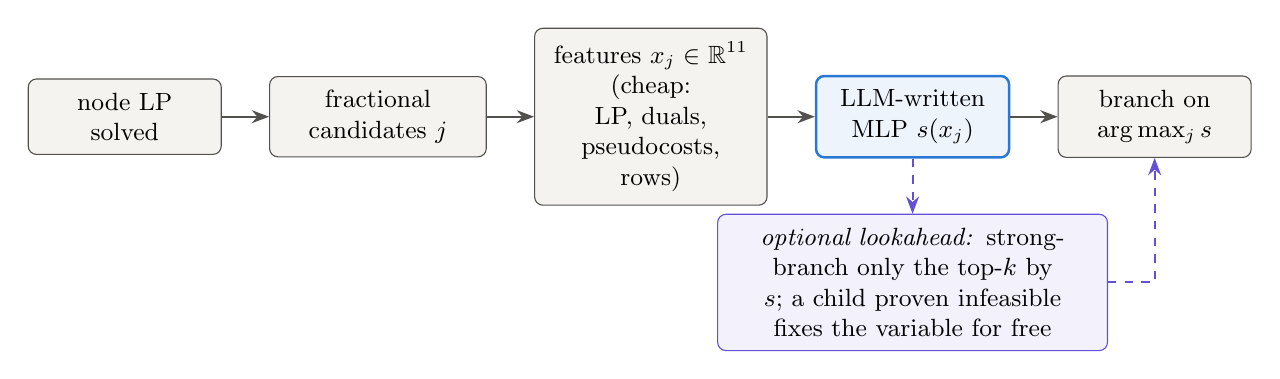
\begin{tikzpicture}[node distance=5mm and 6mm]
\node[box=2.1cm] (lp) {node LP\\ solved};
\node[box=2.4cm, right=of lp] (cand) {fractional\\ candidates $j$};
\node[box=2.6cm, right=of cand] (feat) {features $x_j\in\mathbb{R}^{11}$\\ (cheap: LP, duals,\\ pseudocosts, rows)};
\node[box=2.1cm, hl, right=of feat] (mlp) {LLM-written\\ MLP $s(x_j)$};
\node[box=2.1cm, right=of mlp] (br) {branch on\\ $\arg\max_j s$};
\node[box=4.6cm, draw=look, fill=look!8, below=7mm of mlp] (la) {\emph{optional lookahead:} strong-branch only the top-$k$ by $s$; a child proven infeasible fixes the variable for free};
\draw[arr] (lp) -- (cand); \draw[arr] (cand) -- (feat); \draw[arr] (feat) -- (mlp); \draw[arr] (mlp) -- (br);
\draw[arr, draw=look, dashed] (mlp) -- (la);
\draw[arr, draw=look, dashed] (la.east) -| (br.south);
\end{tikzpicture}
\end{document}
